\documentclass{article}
\usepackage[T1]{fontenc}
\usepackage{graphicx}
\usepackage{listings}
\usepackage{xcolor}
\usepackage{minted}

\graphicspath{ {../img/} }

\begin{document}
    \title{Laboratorium Podstawy Aplikacji Internetowych \\
    Spring}
    \author{Piotr Tylczyński \\
    \texttt{piotr.tylczynski@ptl.cloud}}
    
    \begin{titlepage}
        \maketitle
    \end{titlepage}
    
    \tableofcontents
    \pagebreak
    
    \section{Wstęp}
    Celem tego laboratorium jest pokazanie działanie frameworku Spring w praktyce. Podczas zajęć wykonasz prosty serwer, który obsłuży API dla wypożyczalni samochodów. \\
    Stworzone przez ciebie rozwiązanie będzie bardzo uproszczone w porównaniu do prawdziwych serwerów jakie obsługiwały by takie zadanie. Jednak nie oznacza to że będzie bezużyteczne. Nie licząc braku systemu autoryzacji, stworzysz serwer zgodnie z aktualnymi standardami produkcji takich systemów.
    
    \section{Założenia projektu}
        Tworzymy prosty serwer backendowy służący do obsługi wyporzyczalni samochodów. Chcielibyśmy móc dodawać i usuwać samochody z naszej wyporzyczalni. Oczywiście nie powinno się to dziać zawsze, ale tylko wtedy kiedy nikt z nich nie korzysta - szczególnie ważne w momencie gdy mówimy o usuwaniu auto ze stanu wyporzyczalni. \\
        Dodatkową opcją będzie śledzenie kto, kiedy i co wyprzyczył. Z tego powodu będziemy musieli stworzyć bazę danych klientów.
    
    \section{Inicjalizacja projektu}
        Całość tworzenia kodu rozpoczniemy od stworzenia projektu. W tym celu mamy dwa wyjścia. W pierwszym możemy ręcznie szukać odpowiednich modułów Springa w internecie i repozytoriach \emph{Mavena}. W drugim skorzystamy z rozwiązania Spring Initializr. Trzymając się założeń, że korzystamy z rowiązań wykorzystywanych w przemyśle skorzystamy z Initializr. \\
        Initializr został stworzony w 2013 roku przez firmę VMware, Inc. i jest prostą aplikacją służącą do szybkiego tworzenia baz dla projektów Springa. Możemy w nim wybrać interesujące nas moduły a aplikacja sama zajmie się wyszukaniem ich w repozytoriach Maven i dodaniem odpowiednich wpisów w \emph{pom.xml} jaki i stworzeniem odpowiednich plików w samym projekcie. \\
        Osoby chętne mogą same skorzystać z Initializr i przejść przez kreator. W tym celu należy wskazać moduły:
        \begin{itemize}
            \item Lombok
            \item Spring Web
            \item Spring Data JPA
            \item H2 Database
        \end{itemize}
        Zachęcam jednak do pobrania gotowego prekonfigurowanego repozytorium z linku na końcu skryptu. Pomoże to w uniknięciu prostych błędów i rozbierzności w samej konfiguracji projektu. \\
        Ważnym elementem do rozważenia na tym etapie jest struktura projektu. Spring nie narzuca nic konkretnego, jednak skorzystamy z podejścia jedna funkcjinalność, jeden folder. Pomoże to nam w przyszłości szybko nawigować się po projekcie. Szczególnie jeśli kiedyś zdecydujemy się na jego rozwijanie. Zastanówmy się teraz jakie funkcjonalności mamy do zaimplementowania. Na pewno jest to element zajmujący się klientami, oraz element zajmujący się klientami. Z tego powodu stworzymy dwa foldery. Jeden dedykowany dla kodu obsługującego logikę kilentów i jeden dla logiki aut.
        
        \begin{figure}[h]
            \centering
            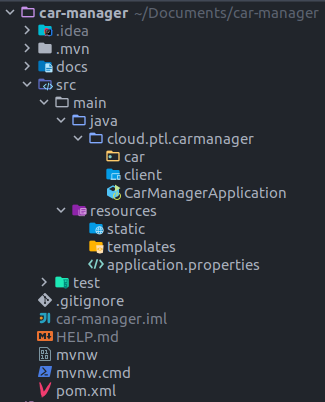
\includegraphics{tree.png}
        \end{figure}
    
    \section{Modelowanie Bazy Danych}
        Najprostszym, jednak bardzo nie efektywnym sposobem będzie ręczne stworzenie schematu bazy danych przez podawanie odpowiednich komend SQL. Następnie do obsługi takiej bazy danych użylibyśmy biblioteki JDBC, tak jak było to pokazywane na zajęciach z Systemów Baz Danych podczas 5 semestru. Jednak jak wspomniałem na początku jest to podejście bardzo nie efektywne. Wyobraźmy sobie, że zamiast modelowania tylko dwóch elementów chcielibyśmy stworzyć ich dwadzieścia. Być może stworzenie bazy danych nie byłoby wyzwaniem, jednak stworzenie i zarządanie skryptami JDBC już tak. Dalej byłoby jeszcze gorzej, ponieważ bazę danych od czasu do czasu trzeba zmieniać, zgodnie ze zmieniającymi się wymaganiami projektu, a to niesie ze sobą potrzebe ręcznego przemodelowania bazy danych a to zmianę skryptów. A na końcu musimy pamiętać, że wiele baz danych posiada swoje charakterystyczne dialekty, co wcale nie ułatwia tworzenia agnostycznego kodu. \\
        Z tego powodu skorzystamy z jednego z modułów, który sami dodaliśmy - Spring Data. Jest to moduł, który za pomocą standardu JPA - Java Persistence API - oraz projektu Hibernate pozwala na modelowanie bazy danych jako obiektów Javy. Hibernate to ORM - Object Relation Mapper. W ten sposób możemy całkowicie zapomnieć o pisaniu czegokolwiek samemu. Od teraz będziemy tworzyć obiekty POJO i odpowiednio je oznaczać a Hibernate zrobi wszystko za nas.
        
        \subsection{Konfigurowanie Bazy Danych}
            Zgodnie z deklaracjami w \emph{pom.xml} będziemy używać bazy danych H2. Jest to proste rozwiązanie w sam raz do celów deweloperskich. Taka baza danych jest włączana za każdym razem, gdy uruchamiamy nasz program i niszczona zaraz po jego zakończeniu. Z tego powodu nie musimy pamiętać o jej ręcznym instalowaniu, włczaniu, wyłączaniu i pielęgnowaniu. \\
            Niestaty jest to też jej duża bolączka, ponieważ za każdym razem gdy wyłączymy nasz program tracimy całą zawartość bazy danych. Na szczeście można to łatwo naprawić - wystarczy podmienić domyślną konfigurację, na taką, która będzie przechowywała dane w plikach. Stracimy w ten sposób na szybkości działania, jednak nie będziemy już tracili danych przy restracie porgramu. \\
            Dodajmy więc do pliku \emph{application.properties} kilka linijek.
            \begin{minted}{properties}
spring.datasource.url=jdbc:h2:file:./db
spring.datasource.driverClassName=org.h2.Driver
spring.datasource.username=sa
spring.datasource.password=admin
spring.jpa.database-platform=org.hibernate.dialect.H2Dialect
spring.jpa.hibernate.ddl-auto=update
spring.h2.console.enabled=true
spring.h2.console.path=/h2
            \end{minted}
            Pierwszych sześć linijek to konfiguracja samego sterownika dla bazy danych. Tak żeby Hibernate wiedział gdzie jest baza, którą ma obsłużyć. Ciekawą rzeczą są dwie ostatnie linijki. Uruchamiają one wbudowany w H2 serwer, który w czasie działania aplikacji pozowli nam na podglądanie bazy danch. Internetową konsolę znajdziemy pod adresem \emph{http://localhost:8080/h2}
        
        \subsection{Obiekty DAO}
            \textbf{DAO} - Data Access Object \\
            To właśnie dzięki nim będziemy mogli modelować naszą bazę. Zwyczajowo, każda klasa opisująca obiekt DAO, kończy się właśnie tym akronimem. 
            \subsubsection{CarDAO}
                Stwórzmy prosty obiekt opisujący samochód.
                \begin{minted}{java}
@Data
@Entity
@Table(name = "car")
public class CarDAO {
    @Id @GeneratedValue(strategy = GenerationType.IDENTITY)
    private Long id;

    private String numberPlate;
    private String seatsNumber;
    private Double totalDistance;
}
                \end{minted}
                \begin{description}
                \item[@Data] adnotacja Lomboka, która automatycznie w czasie kompilacji stworzy gettery, settery, funkcje konwertujące obiekt do stringu, funkcje prównujące obiekty między sobą i wiele innych
                \item[@Entity] wskazuje Springowi, że obiekt będzie trzeba zapisać w bazie danych
                \item[@Table] ustawia nazwę tabeli w bazie danych
                \item[@Id] wskazuje które z pól będzie kluczem głównym relacji
                \item[@GeneratedValue] definiuje w jaki sposób należ tworzyć wartości dla pola $id$. Zwuważmy, że taką adnotację można użyć do dowolnego pola, które będzie mogło być obsłużone przez jakiś skewenser. W naszym przypadku wskazujemy na chęć użycia sekwensera w taki sposób aby każda wartość $id$ była unikalna w całym cyklu życia tabeli   
                \end{description}
            \subsubsection{ClientDAO}
                Teraz twoim zadaniem będzie stworzenie obiektu klienta. Powinie nazywać się \textbf{ClientDAO} i mieć następujące pola:
                \begin{itemize}
                    \item name
                    \item surname
                    \item govID
                \end{itemize}
                Jeśli zrobiłeś wszystko dobrze to powinieneś otrzymać następujący kod
                \begin{minted}{java}
@Entity
@Data
@Table(name = "client")
public class ClientDAO {
    @Id @GeneratedValue(strategy = GenerationType.IDENTITY)
    private Long id;

    private String name;
    private String surname;
    private String govID;
}
            \end{minted}
        \subsubsection{Połączenie CarDAO i ClientDAO}
            W tym momencie mamy dwa osobne obiekty. CarDAO - reprezentujący auto i ClientDAO - reprezentujący klienta. Teraz należałoby stworzyć jakieś połączenie między nimi. Oczywiście takim połączeniem można zarządzać ręcznie, albo skorzystać z możliwości ORM. My skorzystamy z ORM. \\
            Najpierw zastanówmy się jaki typ połączenia należało by wybrać. Zgodnie z logiką chcielibyśmy, aby jeden samochód był wyporzyczony tylko i wyłącznie przez jednego klienta w danym momencie. Natomiast nic nie broni, aby jeden klient wyporzyczał wiele auto naraz. Oznacza to połączenie \textbf{jeden} klient \textbf{do wielu} samochodów. \\
            Dodajmy więc taką informację do obiektów DAO. W klasie CarDAO dopisujemy
            \begin{minted}{java}
@ManyToOne(
        fetch = FetchType.LAZY
)
private ClientDAO rentedBy;
            \end{minted}
            a w klasie ClientDAO
            \begin{minted}{java}
@OneToMany(
        mappedBy = "rentedBy",
        fetch = FetchType.LAZY
)
private Collection<CarDAO> rentedCars;
            \end{minted}
            Ciekawym elementem jest argument $fetch$. Definuje on  w jaki spodób będą pobierane dane z bazy. Zwróćmy uwagę, że zarówno obiekt klienta jak i obiekt samochodu posiadają referencje do siebie nawzajem. Tworzy to stosunkowo niebezpieczną sytuację, w której Hibernate próbowałby pobrać informacje o kliencie, w którym znalazłby referencję do samochdów jakie dany klient wyporzyczył, a w każdym samochodzie znalazłby referencję do osób go wyporzyczających, a w każdej osobie referencję do auto jakie wyporzyczyła i tak tworzymy nieskończoną rekurencję, przepełniamy stos w maszynie wirtualnej (JVM) i crashujemy program. Z tego powodu ustawamy argument $fetch$ na $LAZY$. Oznacza to, że ORM będzie pobierał informacje z bazy danych tylko i wyłącznie gdy program będzie potrzebował do nich dostępu. W ten sposób unikniemy nieskończonej rekurencji. Oczywiście wartość $LAZY$ jest ustawiana przez Spring domyślnie, aby przyspieszyć działanie aplikacji i nie ma potrzeby nadpisywania jej tą samą wartością, jednak zrobiliśmy to, żeby pokazać bardzo poważny problem na jaki niedługo natkniemy się jeszcze raz.
        \subsection{Dostęp do danych}
            Do tej pory zajmowaliśmy się tylko definiowaniem wyglądu bazy danych. Teraz przyjżymy się jak uzyskać dostęp do zgoromadzonych danych. W tym celu skorzystamy z kolejnego udogodnienia modułu Spring Data - czyli repozytoriów. \\
            Są to interfejsy za pomocą, których będziemy definiowali polecenia dla bazy danych. Zauważmy, że w żadnym przypadku nie będziemy używali poleceń SQL. Pozwala to na maksymalną abstrakcję od tego jakiej bazy danych będziemy używali. Aktualnie jest to H2, ale nic nie szkodzi aby podpiąć do naszego projektu MySQL, OracleDB, Postgree, Aurore, albo RedShift.\\
            Zacznijmy od zdefiniowania Repozytorium dla klienta
            \begin{minted}{java}
public interface ClientRepository extends CrudRepository<ClientDAO, Long> {
    Boolean existsByGovID(String govID);
}
            \end{minted}
            a teraz dla pojazdu
            \begin{minted}{java}
public interface CarRepository extends CrudRepository<CarDAO, Long> {
    Boolean existsByNumberPlate(String numberPlate);
    Collection<CarDAO> findAllByRentedBy(ClientDAO clientDAO);
}
            \end{minted}
            Zauważmy, że nie piszemy całych repozytoriów samemu. Rozszerzamy już predefiniwane repozytorium - $CrudRepository$. Znajdują się w nim definicje popularnych poleceń, tworzenie, aktualizacji, usuwania i odczutu danych. Pamiętajmy też, że \textbf{repozytoria nie są klasami tylko interfejsami}. \\
    \section{Logika aplikacji}
        W tym momencie mamy już wszystkie elementy potrzebne do stworzenia logiki naszej aplikacji. Zwyczajowo logikę umieścimy w specjalnych klasach - serwisach. Robi się tak z wielu powodów a niektóre z nich zobaczysz na przykładach w dalszych częściach tego tutorialu. \\
        Stworzymy dwa serwisy, po jednym dla logiki klientów i aut. 
        \subsection{CarService}
        Zacznijmy od serwisu aut - \textbf{CarService}
        \begin{minted}{java}
@Service
public class CarService {
}
        \end{minted}
        Użyliśmy tutaj specjalnej adnotacji $@Service$. Podpowiada on Springowi, że klasa którą piszemy jest specjalnego przeznaczenia - jest serwisem. Spring w czasie uruchamiania aplikacji za każdym razem przegląda wszystkie klasy w celu znalezienia takiej adnotaji. \\
        Jako że piszemy logikę dla samochodu powinniśmy mieć powiązanie z repozytorium odpowiedzialnym za interakcję z samochodami w bazie danych. Dodajmy je.
        \begin{minted}{java}
@Service
public class CarService {
    @Autowired
    private CarRepository carRepository;  
}

        \end{minted}
        Przyjżyj się adnotacji $@Autowired$. Dzięki niej Spring sam w czasie tworzenie obiektów klasy $CarService$ będzie inicjował zmienną $carRepository$ właściwymi wartościami. Po naszej stronie nie musimy już nic robić. Jest to jedna z zalet opisania naszej klasy jako $@Service$. Od teraz możemy korzystać z IoC - Inversion of Controll i DI - dependency injection. Co więcej, teraz nasza klasa serwisu też będzie mogła być wstrzykiwana w taki sam sposób jak repozytorium w każdej klasie zarządzanej przez IoC Springa. \\
        Po zdefiniowaniu wszystkich potrzebnych zmiennych, możemy zacząć pisać właściwą część logiki. Zacznijmy od tworzenia nowych obiektów w bazie danych. Dodajmy funkcję za to odpowiedzialną.
        \begin{minted}{java}
public CarDAO create(CarDAO carDAO){
    return this.carRepository.save(carDAO);
}
        \end{minted}
        Niestety funkcja $CarRepository::save()$ nie potrafi sama określić czy dany obiekt już istnieje w bazie danych czy nie. Dzieje się tak dlatego, że wybraliśmy jako klucz główny sztucznie generowane $id$, a nie numer rejestracji. W momencie gdy wywołujemy tą funkcję, nie znamy jeszcze wartości $id$ - w obiekcie CarDAO ustawialiśmy, że ta wartość ma być zarządzana przez bazę danych. Na szczęście nie jest to problem. Dzięki tworzeniu sztucznego $id$ mamy 100\% pewność, że żadne dwa $id$ się nie zdublują. Rozwiążmy teraz problem sprawdzania, czy dane auto istniej w bazie danych.
        \begin{minted}{java}
private Boolean checkIfExists(CarDAO carDAO){
    if(carDAO.getNumberPlate() == null) return false;
    return
            this.carRepository.existsByNumberPlate(carDAO.getNumberPlate());
}
        \end{minted}
        Na początku sprawdzamy, czy dane auto ma wogóle rejestrację, jak jej nie ma to i tak już nie mamy szans na jego rozpoznanie. Później korzystam z funkcji, którą zdefiniowaliśmy w naszym repozytorium do sprawdzania czy istniją obiekty w bazie danych o podanej rejestracji. Mając obie funkcjie nareszcie możemy stworzyć rozwiązanie, które nie będzie niszczyło naszej bazy przez przypadek, czyli:
        \begin{minted}{java}
public CarDAO createIfNotExits(CarDAO carDAO){
    if(this.checkIfExists(carDAO))
        return carDAO;
    else
        return this.create(carDAO);
}
        \end{minted}
        Z punktu widzenia naszej aplikacji potrzebne są nam jeszcze trzy funkcjonalności - towrzenie nowych aut, wyszukiwanie już istniejących i zarządzanie ich wyporzyczaniem. Zaimplementujmy teraz funkcję odpowiedzialną za wyszukiwanie w bazie danych już istniejących aut.
        \begin{minted}{java}
public CarDAO getOne(Long id) throws Exception {
    Optional<CarDAO> optionalCarDAO =
            this.carRepository.findById(id);
    if(optionalCarDAO.isEmpty())
        throw new ProcessingException("Car not found");
    else return optionalCarDAO.get();
}
        \end{minted}
        Używając funkcji $CarRepository::find()$ otzymujemy specjalny obiekt - $Optional$. Jest to wrapper na dowolny obiekt, który dodatkowo przetrzymuje informację, czy obiekt w nim się znajdujący to przypadkiem nie null. Użyliśmy także specjalnie stworzonego wyjątku - $ProcessingException$. Pomoże nam to w przyszłości tłumaczyć wyjątki rzucane przez Spring do odpowiedzi API. Odejdźmy na chwilę od naszej klasy serwisu i napiszmy właśnie użytą klasę $ProcessingException$
        \begin{minted}{java}
public class ProcessingException extends Exception{
    public ProcessingException(String message){
        super(message);
    }
}
        \end{minted}
        Teraz wróćmy spowrotem do pisanego serwisu i dodajmy dwie ostatnie funkcje - wyporzyczanie samochodu i jego oddawania. Pamiętajmy, że w przechowujemy inforację o całkowitym przebytym dystansie przez każdy samochód i należy go aktualizować w przy każdym oddaniu auta. Zwróćmy też uwagę na zapobieganie oddawania cudzego auta, lub wyporzyczania samochodu już wyporzyczonego.
        \begin{minted}{java}
public CarDAO rent(CarDAO carDAO, ClientDAO clientDAO) throws Exception {
    if (carDAO.getRentedBy() == null){
        carDAO.setRentedBy(clientDAO);
        return this.carRepository.save(carDAO);
    }
    if (carDAO.getRentedBy().equals(clientDAO))
        throw new ProcessingException("Already Rented By You");
    if (carDAO.getRentedBy() != null)
        throw new ProcessingException("Already Rented");
    return null;
}

public CarDAO returnn(CarDAO carDAO, ClientDAO clientDAO, Double distanceCovered) throws Exception {
    if (carDAO.getRentedBy() == null)
        throw new ProcessingException("Car is not rented by anyone");
    if (!carDAO.getRentedBy().equals(clientDAO))
        throw new ProcessingException("Car is not rented by you");
    carDAO.setRentedBy(null);
    carDAO.setTotalDistance(
            carDAO.getTotalDistance() + distanceCovered
    );
        eturn this.carRepository.save(carDAO);
}
        \end{minted}
        W tym momencie skończyliśmy pisanie serwisu odpowiedzialnego za logikę aut.
        \subsection{ClientService}
        Teraz twoim zadaniem jest napisanie podobnego serwisu, ale dla klienta. Wymagane funkcjonalności to:
        \begin{itemize}
            \item dodawanie nowych klientów - $createIfNotExits$
            \item szukanie jednego klienta - $getOne$
            \item wyporzyczanie i oddawanie samochodów - zwróć uwagę, że argumentami funkcji powinny być id auta i klienta + przebyty dystans
        \end{itemize}
        Jeżeli napisałeś wszystko dobrze to twój kod powinien być podobny do tego:
        \begin{minted}{java}
@Service
public class ClientService {
    @Autowired
    private CarService carService;

    @Autowired
    private ClientRepository clientRepository;

    private ClientDAO create(ClientDAO clientDAO){
        if (clientDAO.getRentedCars() == null)
            clientDAO.setRentedCars(new ArrayList<>());
        return this.clientRepository.save(clientDAO);
    }

    private Boolean checkIfExists(ClientDAO clientDAO){
        if (clientDAO.getGovID() == null) return false;
        return this.clientRepository.existsByGovID(clientDAO.getGovID());
    }

    private Boolean checkIfExist(Long id){
        return this.clientRepository.existsById(id);
    }

    public ClientDAO createIfNotExist(ClientDAO clientDAO){
        if (this.checkIfExists(clientDAO))
            return clientDAO;
        else
            return this.create(clientDAO);
    }

    public ClientDAO getOne(Long id) throws Exception {
        Optional<ClientDAO> clientDAOOptional =
                this.clientRepository.findById(id);
        if (clientDAOOptional.isEmpty())
            throw new ProcessingException("Not Found");
        return clientDAOOptional.get();
    }

    public Collection<ClientDAO> findAll(){
        return (Collection<ClientDAO>) this.clientRepository.findAll();
    }

    public ClientDAO rent(CarDAO carDAO, ClientDAO clientDAO) throws Exception {
        this.carService.rent(carDAO, clientDAO);
        return clientDAO;
    }

    public ClientDAO rent(Long carId, Long clientId) throws Exception {
        return this.rent(
                this.carService.getOne(carId),
                this.getOne(clientId)
        );
    }

    public ClientDAO returnn(CarDAO carDAO, ClientDAO clientDAO, Double distanceCovered) throws Exception {
        this.carService.returnn(carDAO, clientDAO, distanceCovered);
        return clientDAO;
    }

    public ClientDAO returnn(Long carId, Long clientId, Double distance) throws Exception {
        return this.returnn(
                this.carService.getOne(carId),
                this.getOne(clientId),
                distance
        );
    }
}
        \end{minted}

    \section{Warstwa Prezentacji}
        Ostatnią rzeczą do wykonania zostaje część programu odpowiedzialna za komunikację z użytkownikiem. Jest to warstwa prezentacji. 
        
\end{document}